
% Template for Elsevier CRC journal article
% version 1.2 dated 09 May 2011

% This file (c) 2009-2011 Elsevier Ltd.  Modifications may be freely made,
% provided the edited file is saved under a different name

% This file contains modifications for Procedia Computer Science
% but may easily be adapted to other journals

% Changes since version 1.1
% - added "procedia" option compliant with ecrc.sty version 1.2a
%   (makes the layout approximately the same as the Word CRC template)
% - added example for generating copyright line in abstract

%-----------------------------------------------------------------------------------

%% This template uses the elsarticle.cls document class and the extension package ecrc.sty
%% For full documentation on usage of elsarticle.cls, consult the documentation "elsdoc.pdf"
%% Further resources available at http://www.elsevier.com/latex

%-----------------------------------------------------------------------------------

%%%%%%%%%%%%%%%%%%%%%%%%%%%%%%%%%%%%%%%%%%%%%%%%%%%%%%%%%%%%%%
%%%%%%%%%%%%%%%%%%%%%%%%%%%%%%%%%%%%%%%%%%%%%%%%%%%%%%%%%%%%%%
%%                                                          %%
%% Important note on usage                                  %%
%% -----------------------                                  %%
%% This file should normally be compiled with PDFLaTeX      %%
%% Using standard LaTeX should work but may produce clashes %%
%%                                                          %%
%%%%%%%%%%%%%%%%%%%%%%%%%%%%%%%%%%%%%%%%%%%%%%%%%%%%%%%%%%%%%%
%%%%%%%%%%%%%%%%%%%%%%%%%%%%%%%%%%%%%%%%%%%%%%%%%%%%%%%%%%%%%%

%% The '3p' and 'times' class options of elsarticle are used for Elsevier CRC
%% Add the 'procedia' option to approximate to the Word template
%\documentclass[3p,times,procedia]{elsarticle}
\documentclass[3p,times]{elsarticle}

%% The `ecrc' package must be called to make the CRC functionality available
\usepackage{ecrc}

%% The ecrc package defines commands needed for running heads and logos.
%% For running heads, you can set the journal name, the volume, the starting page and the authors

%% set the volume if you know. Otherwise `00'
\volume{00}

%% set the starting page if not 1
\firstpage{1}

%% Give the name of the journal
\journalname{Robotics and Computer-Integrated Manufacturing}

%% Give the author list to appear in the running head
%% Example \runauth{C.V. Radhakrishnan et al.}
\runauth{Z. Kootbally and  C. Schlenoff and T. Kramer and S.K. Gupta}

%% The choice of journal logo is determined by the \jid and \jnltitlelogo commands.
%% A user-supplied logo with the name <\jid>logo.pdf will be inserted if present.
%% e.g. if \jid{yspmi} the system will look for a file yspmilogo.pdf
%% Otherwise the content of \jnltitlelogo will be set between horizontal lines as a default logo

%% Give the abbreviation of the Journal.  Contact the journal editorial office if in any doubt
\jid{procs}

%% Give a short journal name for the dummy logo (if needed)
\jnltitlelogo{Robotics and Computer-Integrated Manufacturing}

%% Provide the copyright line to appear in the abstract
%% Usage:
%   \CopyrightLine[<text-before-year>]{<year>}{<restt-of-the-copyright-text>}
%   \CopyrightLine[Crown copyright]{2011}{Published by Elsevier Ltd.}
%   \CopyrightLine{2011}{Elsevier Ltd. All rights reserved}
\CopyrightLine{2014}{Published by Elsevier Ltd.}

%% Hereafter the template follows `elsarticle'.
%% For more details see the existing template files elsarticle-template-harv.tex and elsarticle-template-num.tex.

%% Elsevier CRC generally uses a numbered reference style
%% For this, the conventions of elsarticle-template-num.tex should be followed (included below)
%% If using BibTeX, use the style file elsarticle-num.bst

%% End of ecrc-specific commands
%%%%%%%%%%%%%%%%%%%%%%%%%%%%%%%%%%%%%%%%%%%%%%%%%%%%%%%%%%%%%%%%%%%%%%%%%%

%% The amssymb package provides various useful mathematical symbols
\usepackage{amssymb}


%% The amsthm package provides extended theorem environments
%% \usepackage{amsthm}

%% The lineno packages adds line numbers. Start line numbering with
%% \begin{linenumbers}, end it with \end{linenumbers}. Or switch it on
%% for the whole article with \linenumbers after \end{frontmatter}.
%% \usepackage{lineno}

%% natbib.sty is loaded by default. However, natbib options can be
%% provided with \biboptions{...} command. Following options are
%% valid:

%%   round  -  round parentheses are used (default)
%%   square -  square brackets are used   [option]
%%   curly  -  curly braces are used      {option}
%%   angle  -  angle brackets are used    <option>
%%   semicolon  -  multiple citations separated by semi-colon
%%   colon  - same as semicolon, an earlier confusion
%%   comma  -  separated by comma
%%   numbers-  selects numerical citations
%%   super  -  numerical citations as superscripts
%%   sort   -  sorts multiple citations according to order in ref. list
%%   sort&compress   -  like sort, but also compresses numerical citations
%%   compress - compresses without sorting
%%
%% \biboptions{comma,round}

% \biboptions{}

% if you have landscape tables
\usepackage[figuresright]{rotating}

% put your own definitions here:
%   \newcommand{\cZ}{\cal{Z}}
%   \newtheorem{def}{Definition}[section]
%   ...

% add words to TeX's hyphenation exception list
%\hyphenation{author another created financial paper re-commend-ed Post-Script}

% declarations for front matter
\usepackage{verbatim}
\usepackage{moreverb}                    % for boxedboxedverbatim
\usepackage{fancyvrb}
%\usepackage{stfloats}
\usepackage{subfig}
\usepackage{algpseudocode}
\usepackage[linesnumbered,boxed,ruled]{algorithm2e}

\newenvironment{mylisting}
{\begin{list}{}{\setlength{\leftmargin}{1em}}\item\small}
{\end{list}}

%%-- mytinylisting
\newenvironment{mytinylisting}
{\begin{list}{}{\setlength{\leftmargin}{1em}}\item\tiny\bfseries}
{\end{list}}

\def\cpp{C{}\texttt{++} }

\begin{document}

\begin{frontmatter}

%% Title, authors and addresses

%% use the tnoteref command within \title for footnotes;
%% use the tnotetext command for the associated footnote;
%% use the fnref command within \author or \address for footnotes;
%% use the fntext command for the associated footnote;
%% use the corref command within \author for corresponding author footnotes;
%% use the cortext command for the associated footnote;
%% use the ead command for the email address,
%% and the form \ead[url] for the home page:
%%
%% \title{Title\tnoteref{label1}}
%% \tnotetext[label1]{}
%% \author{Name\corref{cor1}\fnref{label2}}
%% \ead{email address}
%% \ead[url]{home page}
%% \fntext[label2]{}
%% \cortext[cor1]{}
%% \address{Address\fnref{label3}}
%% \fntext[label3]{}

\dochead{}
%% Use \dochead if there is an article header, e.g. \dochead{Short communication}
%% \dochead can also be used to include a conference title, if directed by the editors
%% e.g. \dochead{17th International Conference on Dynamical Processes in Excited States of Solids}

\title{Models Development and Dynamic Generation of PDDL Files for Flexible Kit Building Applications}

%% use optional labels to link authors explicitly to addresses:
%% \author[label1,label2]{<author name>}
%% \address[label1]{<address>}
%% \address[label2]{<address>}

\author[umd]{Z. Kootbally\corref{cor1}}
\ead{zeid.kootbally@nist.gov}
\author[nist]{C. Schlenoff}
\ead{craig.schlenoff@nist.gov}
\author[cua]{T. Kramer}
\ead{thomas.kramer@nist.gov}
\author[mrc]{S.K. Gupta}
\ead{skgupta@umd.edu}

\address[umd]{University of Maryland, College Park, MD 20740, USA}
\address[mrc]{Maryland Robotics Center, University of Maryland, College Park, MD, USA}
\address[nist]{Intelligent Systems Division, National Institute of Standards and Technology, Gaithersburg, MD, USA}
\address[cua]{Department of Mechanical Engineering, Catholic University of America, Washington, DC, USA}


\cortext[cor1]{Corresponding author: Zeid Kootbally, Department of Mechanical Engineering, University of Maryland, College Park, MD 20740, USA}



\begin{abstract}
This paper presents different models that are used to represent PDDL (Planning Domain Definition Language) structures for kit building applications. Moreover, a tool-based approach is described to automatically and dynamically generate PDDL files for replanning from the current state of the world to recover from failures. The effort described in this paper is an attempt at including agility and flexibility into the "Agility Performance of Robotic Systems" project, developed at the National Institute of Standards and Technology (NIST), and conducted in connection with the Working Group on Ontologies for Robotics and Automation
of the IEEE Robotics and Automation Society.
\end{abstract}

\begin{keyword}
PDDL (Planning Domain Definition Language) \sep OWL (Web Language Ontology) \sep knowledge representation \sep robotics \sep XSDL (XML Schema Definition Language)
%% keywords here, in the form: keyword \sep keyword

%% PACS codes here, in the form: \PACS code \sep code

%% MSC codes here, in the form: \MSC code \sep code
%% or \MSC[2008] code \sep code (2000 is the default)

\end{keyword}

\end{frontmatter}

%%
%% Start line numbering here if you want
%%
% \linenumbers

%% main text
\section{Introduction}
\label{s:Introduction}
The new technical idea for the "Agility Performance of Robotic Systems" (APRS) project~\cite{AgilityPerformanceRoboticSystems} at the National Institute of Standards and Technology (NIST) is to develop the measurement science in the form of an integrated agility framework enabling manufacturers to assess and assure the agility performance of their robot systems. This framework includes robot agility performance metrics, information models, test methods, and protocols -- all of which are validated using a combined virtual and real testing environment. The information models enumerate and make explicit the necessary knowledge for achieving rapid re-tasking and being agile and will answer question such as "What does the robot need to know?", "When does it need to know it?", and "How will it get that knowledge?". This framework will (1) allow manufacturers to easily and rapidly reconfigure and re-task robot systems in assembly operations, (2) make robots more accessible to small and medium organizations, (3) provide large organizations greater efficiency in their assembly operations, and (4) allow the U.S. to compete effectively in the global market. Any company that is currently deploying or planning to deploy robot systems will benefit because they will be able to accurately predict the agility performance of their robot systems and be able to quickly re-task and reconfigure their assembly operations.



The increased number of new models and variants have forced manufacturing firms to meet the demands of a diversified customer base by producing products in a short development cycle, yielding low cost, high quality, and sufficient quantity. Modern manufacturing enterprises have two alternatives to face the aforementioned requirements. The first one is to use manufacturing plants with excess capacity and stock of products in inventory to smooth fluctuations in demand. The second one is to use and increase the flexibility of their manufacturing plants to deal with the production volume and variety. While the use of flexibility generates the complexity of its implementation, it still is the preferred solution. Chryssolouris~\cite{Chryssolouris.2005} identified manufacturing flexibility as an important attribute to overcome the increased number of new models and variants from customized demands. Flexibility, however needs to be defined in a quantified fashion before being considered in the decision making process.

Agility is often perceived as combination of speed and flexibility. Gunasekaran~\cite{Gunasekaran.1998} defines agile manufacturing as the capability to survive and prosper in a competitive environment of continuous and unpredictable change by reacting quickly and effectively to changing markets, driven by customer-designed products and services. To be able to respond effectively to changing customer needs in a volatile marketplace means being able to handle variety and introduce new products quickly. Lindbergh~\cite{Lindbergh.1990} and Sharafi \& Zhang~\cite{Sharafi.1999} mentioned that agility consists of flexibility and speed. Essentially, an organisation must be able to \emph{respond flexibly} and \emph{respond speedily}~\cite{Breu.2002}. Conboy \& Fitzgerald~\cite{Conboy.2004} identified terms such as \emph{speed}~\cite{Tan.1998}, \emph{quick}~\cite{DeVor.1995,Kusak.1997,Upton.1994,Yusuf.1999}, \emph{rapid}~\cite{Hong.1996}, and \emph{fast}~\cite{Zain.2003} occur in most definitions of agility.

The above definitions of agile manufacturing can be applied at the assembly level of a manufacturing system. The assembly system needs to have a certain level of flexibility in the presence of disturbances that can be expressed by the degree of robustness. Kannan \& Parker~\cite{Kannan.2006} described robustness as the ability of the system to identify and recover from faults. Robustness of a control system was described by Pinto-Leit\~{a}o \& Restivo~\cite{Leitao.2004} as the capability to remain working correctly and relatively stable, even in presence of disturbances.

The goal of the effort discussed in this paper is to provide a robust architecture for the "Agility Performance of Robotic Systems" project. More particularly, the current effort aims at planning and replanning for failure recovery (e.g., misalignments, incorrect parts and tooling, shortage of parts, or missing tool). Fox \textit{et al.}~\cite{Fox.2006} discussed plan replanning and plan repair when differences are detected between the expected and actual context of execution during plan execution in real environments. The authors define plan repair as the work of adapting an existing plan to a new context while perturbing the original plan as little as possible. Replanning is defined as the work of generating a new plan from scratch.

The planning aspect of the APRS project relies on the Planning Domain Definition Language (PDDL)~\cite{Fox.2003}. In order to operate, the PDDL planners require a PDDL file-set that consists of two files that specify the domain and the problem. From these files, the planning system creates an additional static plan file. Both the domain and problem files are able to be auto-generated from a knowledge representation. The APRS project is working in collaboration with the IEEE Robotics and Automation Society's Ontologies for Robotics and Automation (ORA) Working Group to develop information models related to kitting, including a model of the kitting environment and a model of a kitting plan. Kitting or kit building is a process that brings parts that will be used in assembly operations together in a kit and then moves the kit to the area where the parts are used in the final assembly. It is anticipated that utilization of the knowledge representation will allow for the development of higher performing kitting systems and will lead to the development of agile automated robot assembly. The kitting environment model and the kitting plan model have both been fully defined in each of two languages: XML Schema Definition Language (XSDL)~\cite{Walmsley.2002,XMLschemaPrimer,XMLschemaStructures} and Web Ontology Language (OWL) \cite{OWLoverview,OWLspec,OWLprimer}.


This paper is structured as follows: An overview of the knowledge
driven methodology for the APRS project is presented in Section~\ref{section:architecture}. The XML schemas models that were developed to represent PDDL domain and problem files are discussed in Section~\ref{section:XML}. A java-based tool that was developed to dynamically produce PDDL domain and problem files from the set of OWL files previously generated is described in Section~\ref{section:java-tool}. Finally, concluding remarks and future work are addressed in Section~\ref{section:conclusion}.
\section{Knowledge Driven Methodology}
\label{section:architecture}
\begin{figure}[!htb]
\centering
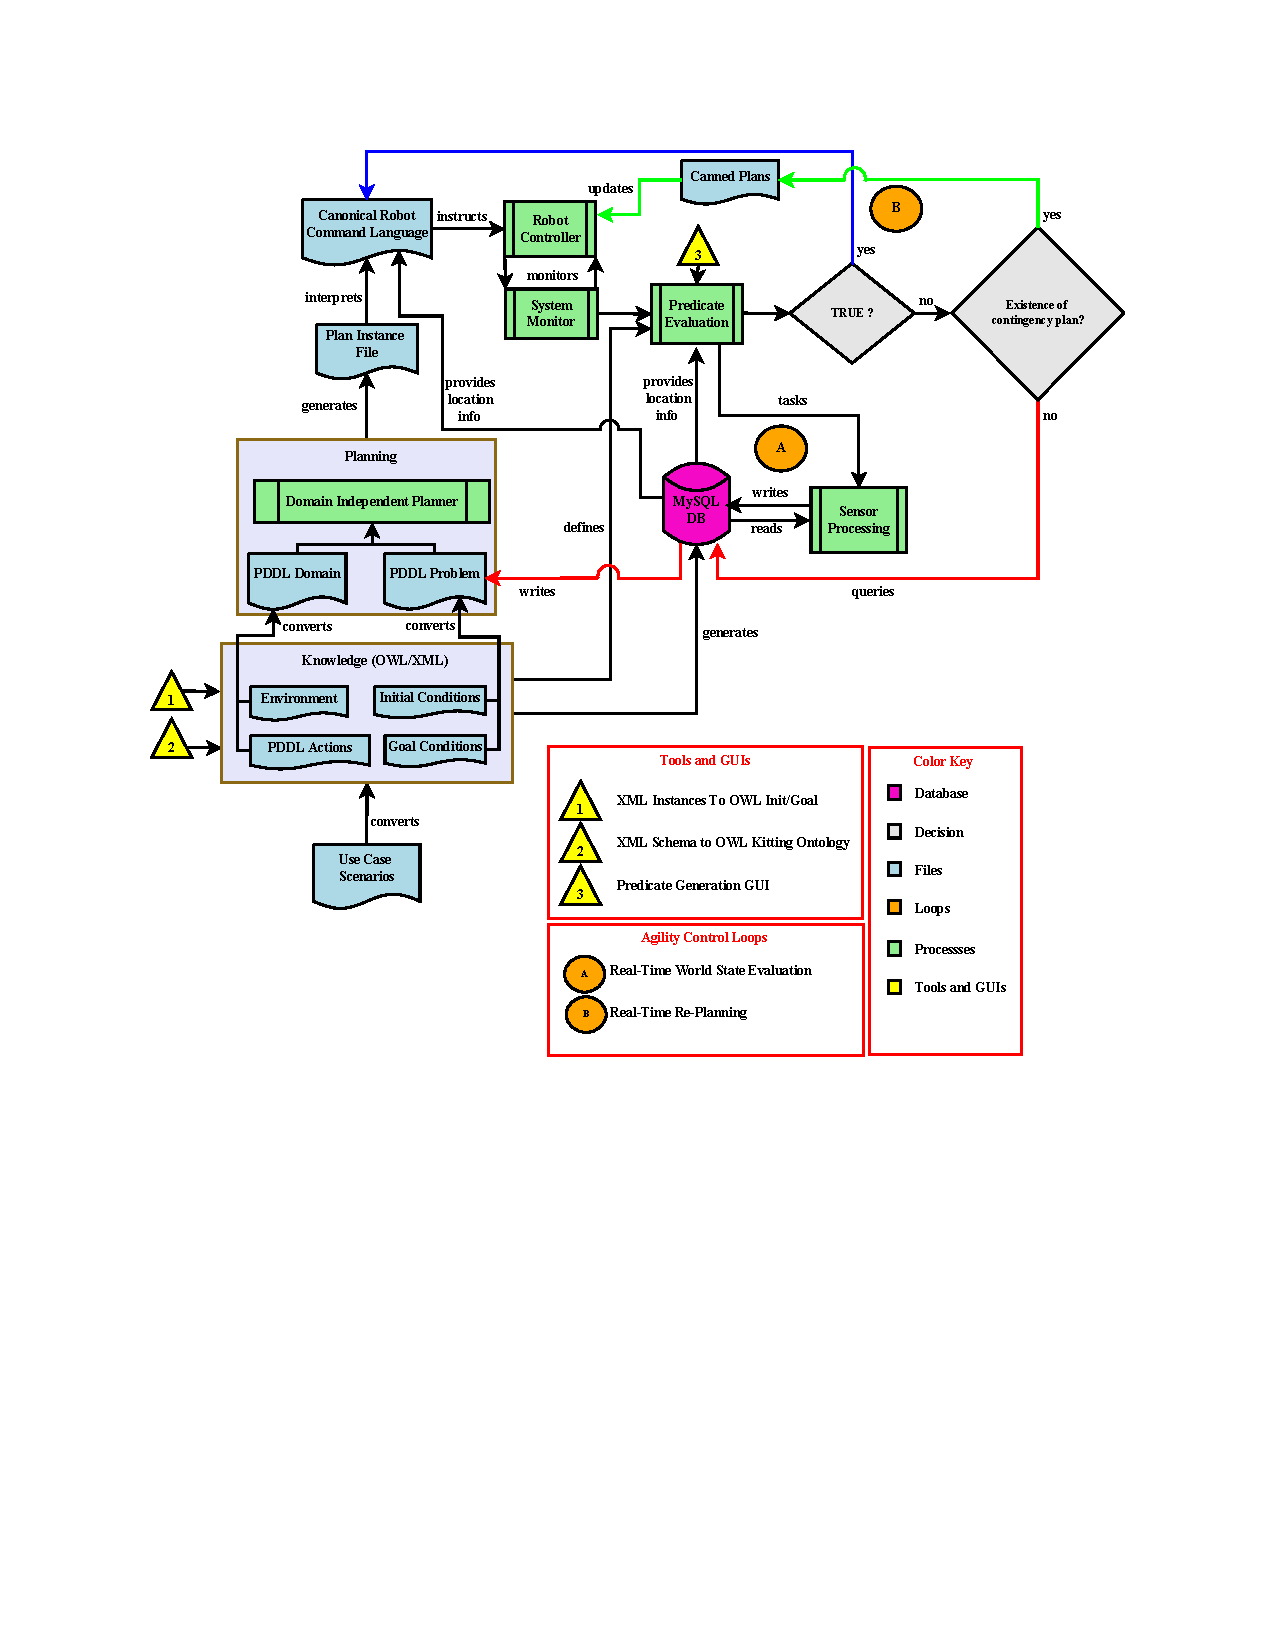
\includegraphics[width=16cm]{images/architecture.pdf}
\caption{Knowledge Driven Design extensions.}
\label{fig:methodology}
\end{figure}
The knowledge driven methodology presented in this section is not purposed to act as a stand-alone system architecture. Rather it is intended to be an extension to well developed hierarchical, deliberative architectures such as 4D/RCS~\cite{Albus2000}. The overall knowledge driven methodology of the system is depicted in Figure~\ref{fig:methodology}. The remainder of this section gives a brief description of the components pertaining to the effort presented in this paper.
\begin{itemize}
\item \textsf{Use Case Scenarios} -- At the early stage of assembly, the \textsf{Use Case Scenarios} define the type of assembly that will be performed. When a new order comes from a customer, an operator enters the specifications of the order in the system via a graphical user interface (e.g., the type of assembly and the number of products required). This first step is therefore an attempt to introduce agility in our system with a functionality that smooths fluctuations in demand.

\item \textsf{Knowledge (OWL/XML)} -- At the next level up, the information encoded in the \textsf{Use Case Scenarios} is then organized into a domain independent representation. The \textsf{Knowledge (OWL/XML)} component contains all of the basic information that was determined to be needed during the evaluation of the \textsf{Use Case Scenarios}. This component consists of class files and instance files that describe the environment and PDDL actions and of instance files that describe the initial and goal states for the current assembly. The knowledge is represented in a compact form with knowledge classes inheriting common attributes from parent classes. The \textsf{PDDL Actions} knowledge describes aspects of PDDL actions that are necessary for the domain under study. The instance files describe the initial and goal states for the system through the \textsf{Initial Conditions} file and the \textsf{Goal Conditions} file, respectively. The initial state file must contain a description of the environment that is complete enough for a planning system to be able to create a valid sequence of actions that will achieve the given goal state. The goal state file only needs to contain information that is relevant to the end goal of the system.

    Since both the OWL and XML implementations of the knowledge representation are file based, real time information proved to be problematic. In order to solve this problem, an automatically generated MySQL database has been introduced as part of the knowledge representation.

\item \textsf{Planning} -- At the next level up, aspects of this knowledge are automatically extracted and encoded in a form that is optimized for a planning system to utilize. The planning language used in the knowledge driven system is expressed with PDDL. The PDDL input format consists of two files that specify the domain and the problem. As shown in Figure~\ref{fig:methodology}, these files are automatically generated from a set of OWL files. The \textsf{PDDL Domain} file is produced from the \textsf{Environment} and the \textsf{PDDL Actions} OWL files while the \textsf{PDDL Problem} file is produced from the \textsf{Initial Condition} and the \textsf{Goal Condition} files. From these two files, a domain independent planning system~\cite{Coles.ICAPS.2010} was used to produce a static \textsf{Plan Instance File}.

\item \textsf{Canonical Robot Command Language} -- Once a plan has been formulated, the knowledge is transformed into a representation that is optimized for use by a robotic system (the Robot
Language). The interpreter combines knowledge from the plan with knowledge from the MySQL database to form a sequence of sequential actions that the robot controller is able to execute. The authors devised a canonical robot command language (CRCL) in which such lists can be written. The purpose of the CRCL is to provide generic commands that implement the functionality of typical industrial robots without being specific either to the language of the planning system that makes a plan or to the language used by a robot controller that executes a plan.

\item \textsf{Robot Controller} -- CRCL commands are then sent to the \textsf{Robot Controller}. One PDDL action from the \textsf{Plan Instance File} is interpreted into a set of CRCL commands. Each set of CRCL commands is queued and where the oldest entry is processed first (FIFO).


\item \textsf{Predicate Evaluation} -- Prior to carrying out the current action, the \textsf{System Monitor} sends the action to a \textsf{Predicate Evaluation} process. The \textsf{Predicate Evaluation} process is used to check if the precondition section for the current PDDL action is true and is intrinsically used to identify failures during the execution of an action by the robot. Each precondition is a predicate expression that must be validated prior to action execution. The world model (the MySQL database) is queried for the pose and class of each relevant parameter of the predicate. The information returned is the latest knowledge that has been recorded by the sensor processing system and is not guaranteed to be up-to-date. This possibly out-of-date information is used as a prediction of the object's current pose and the knowledge is sent as a focus of attention indicator to the sensor processing system. The sensor processing system is instructed to update the world model with current observations and to compute the supporting relationships necessary for predicate evaluation.

    Two distinct results come out of the \textsf{Predicate Evaluation} process. In one hand, all the predicates for the precondition section have been evaluated to true, in this case the robot is signaled to perform the current action. On the other hand, at least one predicate for the precondition section is evaluated to false, therefore a failure occurred in the system. The system provides various known failure modes that could exist for the combination of predicates that were found deficient. It provides the consequences of such a failure occurring, remedial information for such failure (\textsf{Canned Plans}), and the chance that this kind of failure could occur. When no failure modes exist for the failed predicate(s), replanning is performed. Before replanning takes place, the MySQL database is queried in order to build the initial state of the environment in the PDDL problem file. This way ensures that the initial state of the environment is properly set with current information that will be used to generate a new plan. A deeper analysis of the \textsf{Predicate Evaluation} process can be found in~\cite{Balakirsky2013}.


\end{itemize}




\section{Models for PDDL}
\label{section:XML}
This section describes XML schema models that were developed to represent PDDL structures. In this project, a two-step process is required to generate PDDL files. First, XML schema and XML instance files are used to generate a set of OWL files. Then, the generated OWL files are used to produce the PDDL files. The reader may ask about the necessity of the first step and may find it odd that the PDDL files are not directly encoded in OWL by a human expert. Moreover, the reader may ask about the necessity of using OWL as an intermediate step to generate PDDL files.
%The answer for the latter concern is described below while the one for the former concern can be fou

As mentioned in the introductory section, the APRS project is working in collaboration with the ORA Working Group to develop information models related to kitting. Early in its existence, the ORA Working Group made a commitment to use OWL for its models. As the authors used OWL, difficulties arose as summarized in~\cite{Balakirsky.NISTIR.2013}. The models being built lent themselves to a more structured object model approach of the sort used in languages such as EXPRESS~\cite{express}, \cpp classes~\cite{c++}, and XSDL. It was decided to use XSDL  as the language for initial modeling in the APRS project and to produce OWL models from the XSDL models. Moreover, one author already had experience with XSDL and was building \cpp software tools for manipulating XML schemas and instance files. To make the translation work easier and more reliable, additional \cpp tools were built for that purpose.
%In order to maintain compatibility with the IEEE working group, the ontology has been fully defined in OWL.




\subsection{PDDL Background and Structure}
Since its first release in 1998 as the problem-specific language for the AIPS-98 planning competition~\cite{Ghallab.1998}, PDDL has since become a community standard for the representation and exchange of planning domain models. Although the early days of PDDL showed some dissatisfaction in the community, considerable progress was made to the language, thus enabling the comparison between systems sharing the standard and increasing the availability of shared planning resources. The introduction of PDDL has facilitated the scientific development of planning~\cite{Fox.2003}.

PDDL 2.1 is used for the effort presented in this paper. PDDL 2.1 offers a revised version from the original version of the syntax for expressing numeric-valued fluents. Gerevini \textit{et al.}~\cite{Gerevini.2008} define a numeric fluent as a state variable over the set $\mathbb{R}$ of real numbers such that there exists at least one domain action that can change its initial value specified in the problem initial state. Fox \& Long~\cite{Fox.2003} proposed a definitive syntax for the expression of numeric fluents. The authors provided some minor revisions to the version proposed by McDermott~\cite{Mcdermott.2000}. Another feature introduced in PDDL 2.1 as an optional field within the specification of problems is a plan metric. Plan metrics specify the basis on which a plan will be evaluated for a given problem. Different optimal plans can be produced with different plan metrics for the same initial and goal states. The use of PDDL 2.1 for the effort presented in this paper was motivated by numeric fluents and plan metrics. Even though plan metrics is not currently used in our effort, it is the intention of the authors to do so as the project grows.


\subsubsection{PDDL Domain File}
\label{ss:PDDLdomainFile}
Prior the development of a schema model, components of PDDL domain and problem files need to be identified. Figure~\ref{fig:domain} is an excerpt of the PDDL domain file created for kitting. This excerpt is used only for the purpose of this paper. The complete PDDL domain file for kitting consists of 12 \textsf{types}, 34 \textsf{predicates}, 9 \textsf{functions}, and 10 \textsf{actions}.

\begin{figure}[t!h!]
\begin{minipage}{.5\paperwidth}
\begin{mylisting}
\begin{Verbatim}[commandchars=\\\{\},fontsize=\footnotesize, numbers=left, numbersep=2pt]
(define (domain kitting-domain)
    (:requirements :strips :typing :derived-predicates :action-costs :fluents :equality)
    (:types
        EndEffector EndEffectorHolder Kit KitTray
        LargeBoxWithEmptyKitTrays LargeBoxWithKits
        Part PartsTray EndEffectorChangingStation
        Robot StockKeepingUnit WorkTable)

    (:predicates
        (hasEndEffector-HeldObject-None ?endeffector - EndEffector)
        (hasEndEffector-For-Sku-KitTray ?endeffector - EndEffector ?sku - StockKeepingUnit)
        (hasRobot-EndEffector ?robot - Robot ?endeffector - EndEffector)	
        (hasEndEffector-PhysicalLocation-RefObject-Robot ?endeffector - EndEffector
                                                         ?robot - Robot)	
        (hasKitTray-SkuObject-Sku ?kittray - KitTray ?sku - StockKeepingUnit)
        (hasKitTray-PhysicalLocation-RefObject-LBWEKT ?kittray - KitTray
                                                      ?lbwekt - LargeBoxWithEmptyKitTrays)
        (hasEndEffector-HeldObject-KitTray ?endeffector - EndEffector ?kittray - KitTray)
        (hasKitTray-PhysicalLocation-RefObject-EndEffector ?kittray - KitTray
                                                           ?endeffector - EndEffector))

    (:functions
        (quantity-of-parts-in-partstray ?partstray - PartsTray)
        (quantity-of-parts-in-kit ?sku - StockKeepingUnit ?kit - Kit)
        (quantity-of-kittrays-in-lbwekt ?lbwekt - LargeBoxWithEmptyKitTrays)
        (quantity-of-kits-in-lbwk ?lbwk - LargeBoxWithKits)
        (current-quantity-kit ?kit - Kit)
        (final-quantity-kit ?kit - Kit)
        (capacity-of-parts-in-kit ?partsku - StockKeepingUnit ?kit - Kit)
        (capacity-of-kits-in-lbwk ?lbwk - LargeBoxWithKits)
        (part-found-flag))

    (:action Take-KitTray
        :parameters(
            ?robot - Robot
            ?kittray - KitTray
            ?lbwekt - LargeBoxWithEmptyKitTrays
            ?endeffector - EndEffector
            ?sku - StockKeepingUnit)
        :precondition(and
            (> (quantity-of-kittrays-in-lbwekt ?lbwekt) 0)
            (hasEndEffector-HeldObject-None ?endeffector)
            (hasEndEffector-For-Sku-KitTray ?endeffector ?sku)
            (hasRobot-EndEffector ?robot ?endeffector) 					
            (hasEndEffector-PhysicalLocation-RefObject-Robot ?endeffector ?robot)		
            (hasKitTray-SkuObject-Sku ?kittray ?sku)
            (hasKitTray-PhysicalLocation-RefObject-LBWEKT ?kittray ?lbwekt))	
        :effect(and
            (decrease (quantity-of-kittrays-in-lbwekt ?lbwekt) 1)
            (hasEndEffector-HeldObject-KitTray ?endeffector ?kittray) 				
            (hasKitTray-PhysicalLocation-RefObject-EndEffector ?kittray ?endeffector) 	
            (not (hasEndEffector-HeldObject-None ?endeffector)) 				
            (not (hasKitTray-PhysicalLocation-RefObject-LBWEKT ?kittray ?lbwekt))))
)

\end{Verbatim}
\end{mylisting}
\end{minipage}
\caption{Excerpt of the PDDL domain file for kitting.}
\label{fig:domain}
\end{figure}

The different components of a PDDL domain file are described below:
\begin{itemize}
\item line 1: The keyword \textsf{domain} signals a planner that this file contains information on the domain. \textsf{kitting-domain} is the name given to the domain in the example.
\item line 2: It can be seen in the example that PDDL includes a syntactic representation of the level of expressivity required in particular domain descriptions through the use of \textsf{requirements} flags. This gives the opportunity for a planning system to reject attempts to plan with domains that make use of more advanced features of the language than the planner can handle.

\item lines 3--7:  Parameter and object types have to be declared before they are used (before \textsf{predicates} and \textsf{functions}). This is done with the declaration \textsf{(:types $name_1$ ... $name_n$)}.
\item lines 9--20: The \textsf{predicates} part of a domain definition specify only what are the predicate names used in the domain, and their number of arguments (and argument types, if the domain uses \textsf{typing}). The ``meaning'' of a predicate, in the sense of for what combinations of arguments it can be true and its relationship to other predicates, is determined by the effects that actions in the domain can have on the predicate, and by what instances of the predicate are listed as true in the initial state of the problem definition.
\item lines 22--31: \textsf{functions} are used to declare numeric fluents. Numeric assignments (initial value of each function) are set in the initial state of the problem file and change when an action is executed. The declaration of functions is similar to predicates.
\item lines 33--53: The domain definition contains operators (called \textsf{actions} in PDDL). An action statement specifies a way that a planner affects the state of the world. The statement includes \textsf{parameters}, \textsf{preconditions}, and \textsf{effects}. An \textsf{action} is identified by a unique name (\textsf{Take-KitTray} at line 33). Each \textsf{parameter} of an \textsf{action} consists of a name and a type (e.g., at line 35, \textsf{robot} is the name of the parameter and \textsf{Robot} is its type). \textsf{Preconditions} and \textsf{effects} may consist of positive predicates (lines 42--47 and lines 50--51), function operations (line 49), and conditions on numeric expressions (line 41). Conditions on numeric expressions are always comparisons between pairs of numeric expressions. \textsf{Effects} may also consist of negative predicates (lines 52--53).

\end{itemize}

\subsubsection{PDDL Problem File}
Figure~\ref{fig:problem} is a complete PDDL problem file created for kitting. The different components of a PDDL problem file are described below:

\begin{figure}[h!t!]
\begin{minipage}{.5\paperwidth}
\begin{mylisting}
\begin{Verbatim}[commandchars=\\\{\},fontsize=\footnotesize, numbers=left, numbersep=2pt]
(define (problem kitting-problem)
    (:domain kitting-domain)
    (:objects
        robot_1 - Robot
        changing_station_1 - EndEffectorChangingStation
        kit_tray_1 - KitTray
        kit_1 - Kit
        empty_kit_tray_supply - LargeBoxWithEmptyKitTrays
        finished_kit_receiver - LargeBoxWithKits
        work_table_1 - WorkTable
        part_a_tray part_b_tray - PartsTray
        part_a_1 part_a_2 part_b_1 - Part
        part_gripper tray_gripper - EndEffector
        part_gripper_holder tray_gripper_holder - EndEffectorHolder
        stock_keeping_unit_part_a stock_keeping_unit_part_b - StockKeepingUnit)
    (:init
        (hasPart-SkuObject-Sku part_a_1 stock_keeping_unit_part_a)
        (hasPart-SkuObject-Sku part_a_2 stock_keeping_unit_part_a)
        (hasPart-SkuObject-Sku part_b_1 stock_keeping_unit_part_b)
        (hasKit-KitTray kit_1 kit_tray_1)
        (hasKitTray-SkuObject-Sku kit_tray_1 stock_keeping_unit_kit_tray)
        (hasEndEffector-PhysicalLocation-RefObject-EndEffectorHolder part_gripper part_gripper_holder)
        (hasEndEffector-PhysicalLocation-RefObject-EndEffectorHolder tray_gripper tray_gripper_holder)
        (hasRobot-No-EndEffector robot_1)
        (hasWorkTable-ObjectOnTable-None work_table_1)
        (hasKitTray-PhysicalLocation-RefObject-LBWEKT kit_tray_1 empty_kit_tray_supply)	
        (hasPart-PhysicalLocation-RefObject-PartsTray part_a_1 part_a_tray)
        (hasPart-PhysicalLocation-RefObject-PartsTray part_a_2 part_a_tray)
        (hasPart-PhysicalLocation-RefObject-PartsTray part_b_1 part_b_tray)
        (hasEndEffector-HeldObject-None part_gripper)
        (hasEndEffector-HeldObject-None tray_gripper)
        (hasPartsVessel-Part part_a_tray part_a_1)
        (hasPartsVessel-Part part_a_tray part_a_2)
        (hasPartsVessel-Part part_b_tray part_b_1)
        (hasEndEffector-For-Sku-KitTray tray_gripper stock_keeping_unit_kit_tray)
        (hasEndEffector-For-Sku-Part part_gripper stock_keeping_unit_part_a)
        (hasEndEffector-For-Sku-Part part_gripper stock_keeping_unit_part_b)
        (hasEndEffectorHolder-EndEffector part_gripper_holder part_gripper)
        (hasEndEffectorHolder-EndEffector tray_gripper_holder tray_gripper)
        (hasEndEffectorHolder-PhysicalLocation-RefObject-ChangingStation part_gripper_holder changing_station_1)
        (hasEndEffectorHolder-PhysicalLocation-RefObject-ChangingStation tray_gripper_holder changing_station_1)
        (hasEndEffectorChangingStation-EndEffectorHolder changing_station_1 part_gripper_holder)
        (hasEndEffectorChangingStation-EndEffectorHolder changing_station_1 tray_gripper_holder)
        (= (quantity-of-parts-in-partstray part_a_tray) 2)
        (= (quantity-of-parts-in-partstray part_b_tray) 1)
        (= (quantity-of-parts-in-kit stock_keeping_unit_part_a kit_1) 0)
        (= (quantity-of-parts-in-kit stock_keeping_unit_part_b kit_1) 0)
        (= (quantity-of-kittrays-in-lbwekt empty_kit_tray_supply) 1)
        (= (quantity-of-kits-in-lbwk finished_kit_receiver) 0)
        (= (capacity-of-kits-in-lbwk finished_kit_receiver) 12)
        (= (current-quantity-kit kit_1) 0)
        (= (final-quantity-kit kit_1) 3)
        (= (part-found-flag) 1))
    (:goal(and
        (= (capacity-of-parts-in-kit stock_keeping_unit_part_a kit_1) 2)
        (= (capacity-of-parts-in-kit stock_keeping_unit_part_b kit_1) 1)
        (hasKit-PhysicalLocation-RefObject-LBWK kit_1 finished_kit_receiver)
        (hasLBWK-Kit finished_kit_receiver kit_1)))
)
\end{Verbatim}
\end{mylisting}
\end{minipage}
\caption{The PDDL problem file for kitting.}
\label{fig:problem}
\end{figure}


\begin{itemize}
\item line 1: The keyword \textsf{problem} signals a planner that this file contains information on the problem. \textsf{kitting-problem} is the name given to the problem in the example.
\item line 2: The keyword \textsf{domain} is a reference to the domain to which the problem is associated. In the example, the domain refers to the domain described in Figure~\ref{fig:domain}.
\item lines 3--17:  \textsf{objects} specifies the distinct types of objects that will appear in the initial and goal states.
\item lines 18--57: The \textsf{init} section consists of predicates that are true in the initial state. Because of the closed assumption of PDDL, predicates not specified in the \textsf{init} section are set to false. The initial value of each \textsf{function} described in the domain is also set in the \textsf{init} section. For instance, line 43 tells the planner that \textsf{kit\_1} has the capacity of holding only 1 part of type \textsf{stock\_keeping\_unit\_part\_c}. In Figure~\ref{fig:problem}, function assignments are depicted at lines 40--57.
\item lines 58--62: The \textsf{goal} section specifies the predicates that need to be true in the goal state. The value that a \textsf{function} needs to reach may also be specified in the \textsf{goal} section.
\end{itemize}

\subsection{Models for PDDL Domain}
A closer look at Figure~\ref{fig:problem} shows that all the basic components (objects, predicates, and functions) in the problem are also defined in the domain. The only difference is that the problem requires instance parameters while the domain uses generic parameters. Therefore, only the PDDL domain needs to be modeled and the information that goes in the definition of the problem can be mapped in the program. The authors have modeled the structure of a PDDL domain in the SOAP schema. SOAP stands for States, Ordering constructs, Actions, and Predicates. To remove any confusion on this acronym, the authors need to clarify that models of states, ordering constructs, actions, and predicates were used in a sister project, that is, the SOAP model discussed in this section is used in multiple projects.


The \textsf{types} section in the domain and the \textsf{objects} section in the problem are stored in the KittingWorkstation model and this model is imported in the SOAP model. \textsf{SolidObject} and \textsf{DataThing} constitute the two top-level classes of the KittingWorkstation ontology model, from which all other classes are derived. \textsf{SolidObject} models solid objects, things made of matter. The KittingWorkstation ontology includes several subclasses of \textsf{SolidObject} that are formed from components that are \textsf{SolidObject}. The \textsf{DataThing} class models data for \textsf{SolidObject}. The KittingWorkstation model is fully documented in~\cite{Balakirsky.NISTIR.2013}.

Conceptually, the SOAP and KittingWorkstation models are object models as found in several object oriented programming languages (\cpp, for example~\cite{c++}). That is:
\begin{itemize}
\item the model consists primarily of class definitions,
\item a class defines a type of thing,
\item classes have attributes ("elements" in XML schema language),
\item the class definition gives the class (or data type for
individual variables) of each attribute,
\item some attributes may occur optionally or multiple times,
\item some classes are derived from others; thus, there is a
derivation hierarchy,
\item a derived class has all the attributes of its parent plus,
possibly, some of its own,
\item if class B is derived from class A, then if the type of
an attribute is class A, an instance of class B may be
used as the value of the attribute,
\item the model does not use multiple inheritance,
\item the model also uses primitive data types such as numbers and strings, and provides for defining specialized data types by putting constraints on primitive data types.
\end{itemize}



To describe the SOAP model for PDDL domains, the authors will refer to Figure~\ref{fig:domain}. The different figures of classes presented in the remainder of this section were generated by XMLSpy~\cite{XMLSpyManual}. In these figures, a dotted line around a box means the attribute is optional (may occur zero times), a $0..\infty$ underneath a box means it may not occur, with no upper limit on the number of occurrences, and a $1..\infty$ underneath a box means it may occur at least once, with no upper limit on the number of occurrences.


\paragraph{Domain} \textsf{DomainType} extends \textsf{DataThingType} and consists of a \textsf{Name} (inherited from \textsf{DataThingType}), a set of requirements (\textsf{Requirement}), a set of variables (\textsf{Variable}), a set of predicates (\textsf{PositivePredicateType}), an optional set of functions (\textsf{FunctionType}), and a set of actions (\textsf{ActionBaseType}). These components consist a PDDL domain file such as the one showed in Figure~\ref{fig:domain}. A \textsf{Requirement} and a \textsf{Variable} are of type \texttt{xs:NMTOKEN} in XSDL and of type \texttt{string} in OWL. The other components are described later in this section.

\begin{figure}[htb!]
\centering
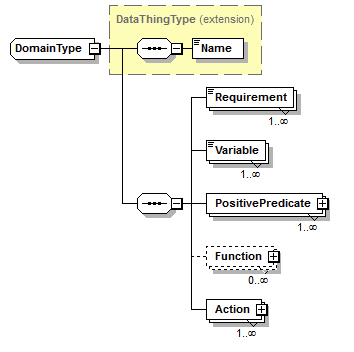
\includegraphics[width=8cm]{images/soap/DomainTypeMinimal.png}
\caption{Domain model.}
\label{fig:DomainType}
\end{figure}

\paragraph{Predicate}
PDDL predicates are represented in a positive and negative forms. Figure~\ref{fig:domain} contains both positive (e.g., line 42) and negative predicates (e.g., lines 10 and 53).
A PDDL positive predicate is modeled with \textsf{PositivePredicateType}, which is depicted in Figure~\ref{fig:PositivePredicateType}. A \textsf{PositivePredicateType} extends \textsf{DataThingType} and consists of a name (\textsf{Name}) that is inherited, an optional description (\textsf{Description}), a reference parameter (\textsf{ReferenceParameter}), and an optional target parameter (\textsf{TargetParameter}). The predicates used in the kitting PDDL domain and problem files all have at least one parameter and can have up to two parameters. In the case a predicate has two parameters, the first parameter is identified as a reference parameter (\textsf{ReferenceParameter}) and the second parameter is identified as the target parameter (\textsf{TargetParameter}). In the case a predicate has only one parameter, this parameter is identified as the reference parameter (\textsf{ReferenceParameter}).
\begin{figure}[htb!]
\centering
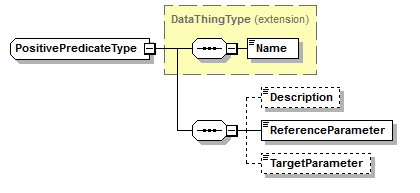
\includegraphics[width=8cm]{images/soap/PositivePredicateType.png}
\caption{Positive predicate model.}
\label{fig:PositivePredicateType}
\end{figure}

\paragraph{Function}
PDDL functions are represented by \textsf{FunctionType}. The structure of \textsf{FunctionType} is illustrated in Figure~\ref{fig:FunctionType}. The interpretation for  \textsf{ReferenceParameter} and for \textsf{TargetParameter} are the same as the ones given earlier. As one can see,  \textsf{ReferenceParameter} and \textsf{TargetParameter} are both optional for a \textsf{FunctionType} since some PDDL functions in our kidding domain are void of parameters (e.g., \textsf{(part-found-flag)} in Figure~\ref{fig:domain}).

\begin{figure}[htb!]
\centering
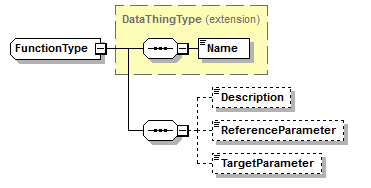
\includegraphics[width=8cm]{images/soap/FunctionType.png}
\caption{Function model.}
\label{fig:FunctionType}
\end{figure}

\newpage
\begin{figure}[htb!]
\centering
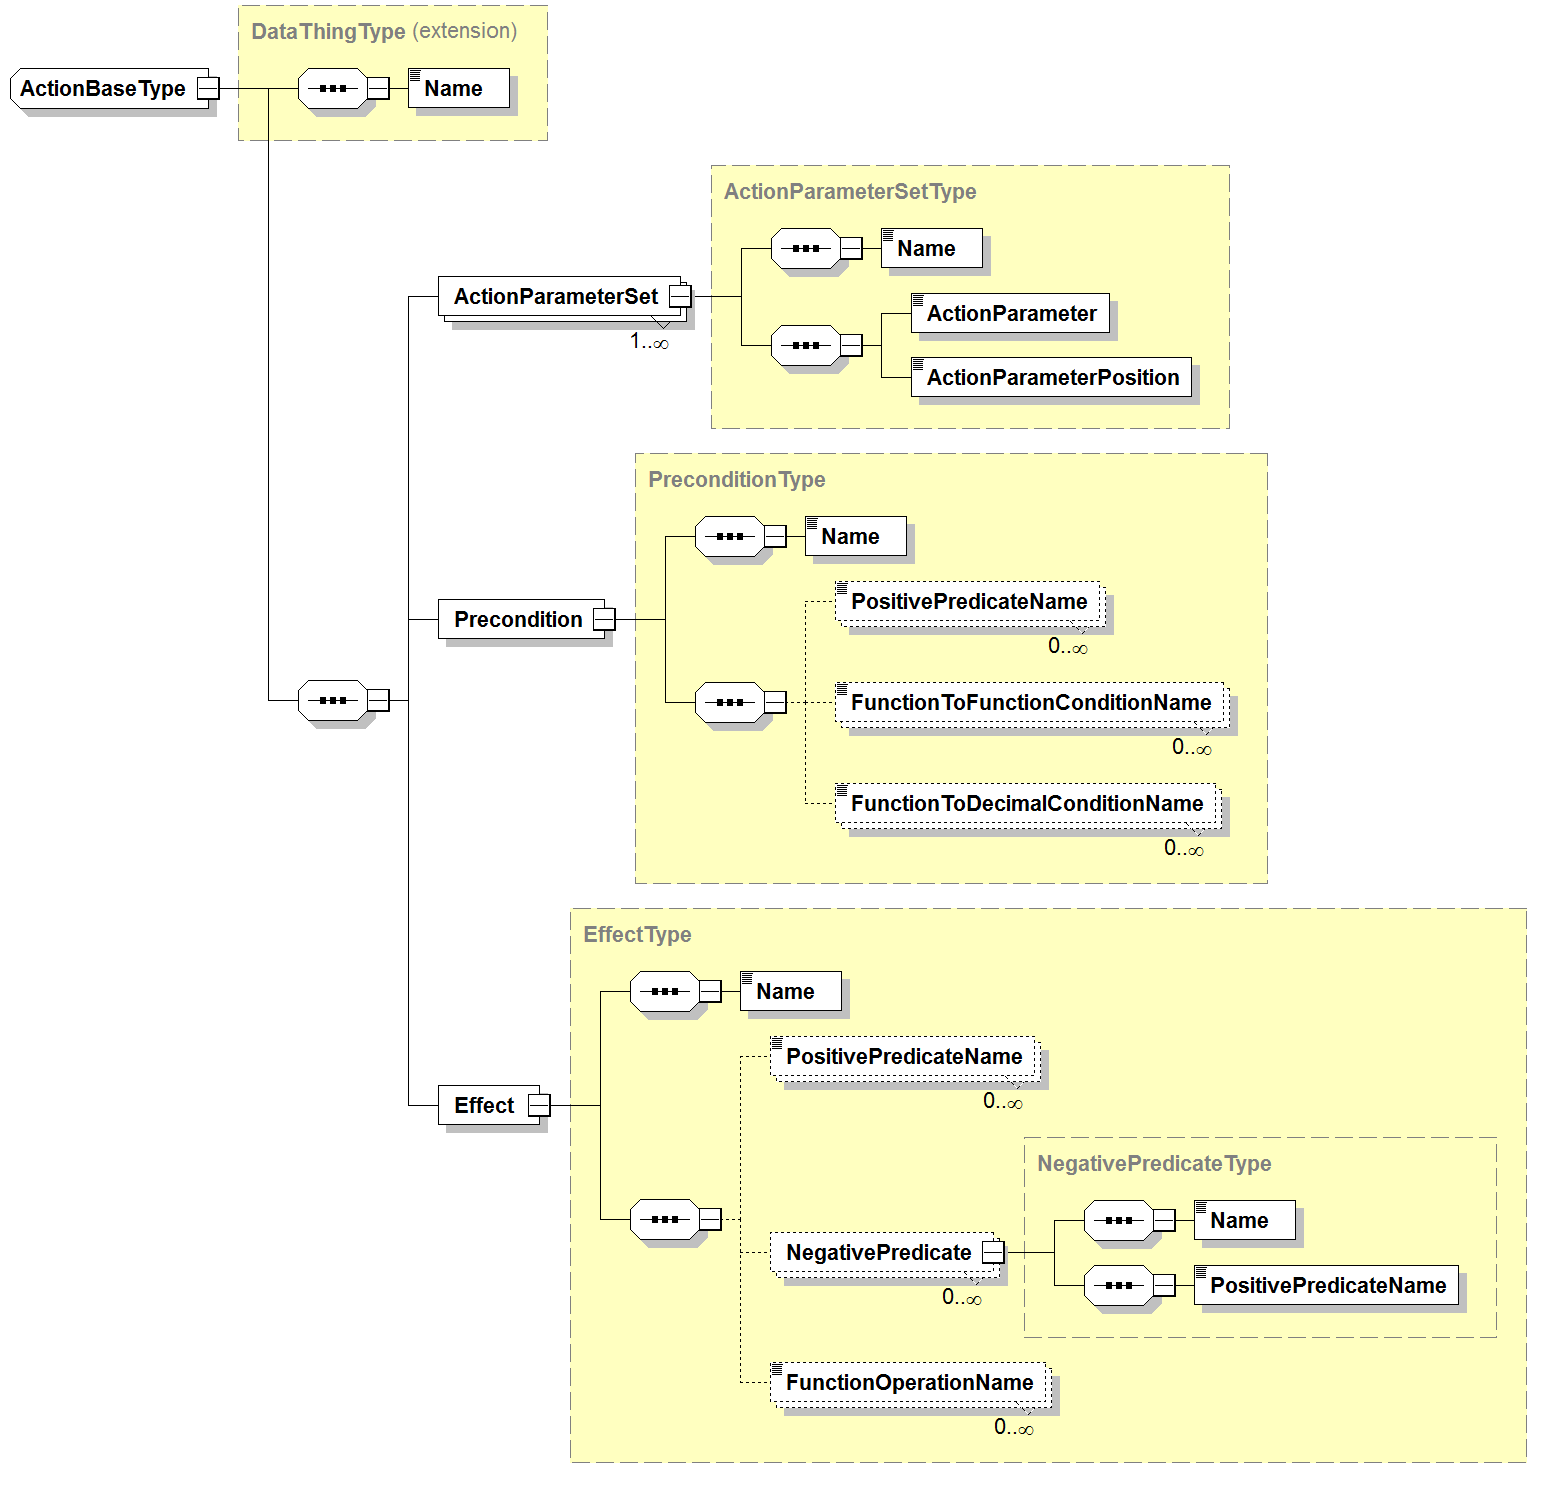
\includegraphics[width=15cm]{images/soap/ActionBaseType.png}
\caption{Action model.}
\label{fig:ActionBaseType}
\end{figure}


\begin{figure}[htb!]
\centering
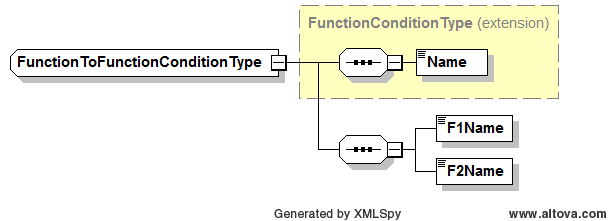
\includegraphics[width=8cm]{images/soap/FunctionToFunctionConditionType.png}
\caption{Function to function condition model.}
\label{fig:FunctionToFunctionConditionType}
\end{figure}


\begin{figure}[htb!]
\centering
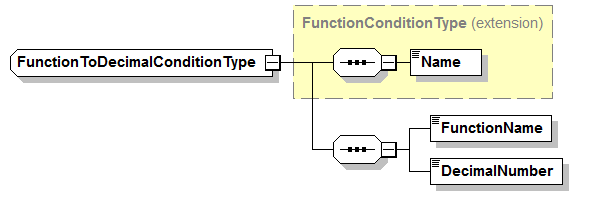
\includegraphics[width=8cm]{images/soap/FunctionToDecimalConditionType.png}
\caption{Function to decimal condition model.}
\label{fig:FunctionToDecimalConditionType}
\end{figure}
\paragraph{Action}
As mentioned in Section~\ref{ss:PDDLdomainFile}, a PDDL action consists of a unique name, a set of parameters, a precondition section, and an effect section. The model for PDDL actions is \textsf{ActionBaseType} (Figure~\ref{fig:ActionBaseType}). \textsf{ActionBaseType} extends \textsf{DataThingType}. The models for the components of a PDDL action are described as follows:
\begin{itemize}
\item  The unique name of a PDDL action is assigned with the inherited \textsf{Name} attribute.
\item PDDL actions' parameters are represented with \textsf{ActionParameterSetType}. An \textsf{ActionParameterSetType} consists of a unique \textsf{Name}, \textsf{ActionParameter} is a text field (\textsf{xs:NMTOKEN} in XSDL) which represents the type of the parameter, and \textsf{ActionParameterPosition} is an integer (\textsf{xs:positiveInteger} in XSDL) which represents the position of the \textsf{ActionParameter} in the list of parameters for a PDDL action \footnote{The authors are currently using numbers (integers) to represent orders of parameters in a list of parameters as no built-in structure exists for the representation of ordered list in OWL.}. To illustrate these components, the reader may refer to Figure~\ref{fig:domain} (line 33).  The action \textsf{Take-KitTray} consists of five parameters. Each parameter of the action \textsf{Take-KitTray}  is an \textsf{ActionParameterSetType}.  The \textsf{ActionParameter} for the parameter \textsf{robot} is \textsf{Robot} and its  \textsf{ActionParameterPosition}  is 1.
\item The precondition section of a PDDL action is modeled with \textsf{PreconditionType} . A \textsf{PreconditionType} extends \textsf{DataThingType}. A \textsf{PreconditionType} consists of a unique \textsf{Name} (inherited), optional references to positive predicates (\textsf{PositivePredicateType}),  optional references to conditions on functions (\textsf{FunctionConditionType}). A \textsf{FunctionConditionType} is a comparison between pairs of numeric expressions. It includes a function to function condition model and a function to decimal condition model.
\begin{itemize}
\item A function to function condition model (\textsf{FunctionToFunctionConditionType}) is represented in Figure~\ref{fig:FunctionToFunctionConditionType}. The model extends \textsf{FunctionConditionType} and consists of a \textsf{Name} (inherited from \textsf{DataThing}), a reference to the first \textsf{FunctionType} (\emph{F1Name}), and a reference to the second \textsf{FunctionType} (\emph{F2Name}). Comparisons between \textsf{FunctionType}s require definitions of mathematical symbols. Specific mathematical symbols ($<$, $\leq$, $=$, $\geq$, $>$) are expressed with subtypes of \textsf{FunctionConditionType}. The subtypes are \textsf{FunctionToFunctionLessType} (Figure~\ref{fig:FunctionToFunctionLessType}), \textsf{FunctionToFunctionLessOrEqualType} (Figure~\ref{fig:FunctionToFunctionLessOrEqualType}), \textsf{FunctionToFunctionEqualType} (Figure~\ref{fig:FunctionToFunctionEqualType}), \textsf{FunctionToFunctionGreaterOrEqualType} (Figure~\ref{fig:FunctionToFunctionGreaterOrEqualType}), and \textsf{FunctionToFunctionGreaterType} (Figure~\ref{fig:FunctionToFunctionGreaterType}).
\item A function to decimal condition model (\textsf{FunctionToDecimalConditionType}) is represented in Figure~\ref{fig:FunctionToDecimalConditionType}. The model extends \textsf{FunctionConditionType} and consists of a \textsf{Name} (inherited from \textsf{DataThing}), a reference to a \textsf{FunctionType} (\emph{FunctionName}), and a decimal value (\emph{DecimalNumber}). As for \textsf{FunctionToFunctionConditionType}, subtypes of \textsf{FunctionToDecimalConditionType} indicates the type of the comparison between a function and a decimal number. The subtypes of \textsf{FunctionToDecimalConditionType} are \textsf{FunctionToDecimalLessType} (Figure~\ref{fig:FunctionToDecimalLessType}), \textsf{FunctionToDecimalLessOrEqualType} (Figure~\ref{fig:FunctionToDecimalLessOrEqualType}), \textsf{FunctionToDecimalEqualType} (Figure~\ref{fig:FunctionToDecimalEqualType}), \textsf{FunctionToDecimalGreaterOrEqualType} (Figure~\ref{fig:FunctionToDecimalGreaterOrEqualType}), and \textsf{FunctionToDecimalGreaterType} (Figure~\ref{fig:FunctionToDecimalGreaterType}).

    An illustration of a \textsf{FunctionToDecimalGreaterType} is given at line 41 in Figure~\ref{fig:domain}. \textsf{($>$ (quantity-of-kittrays-in-lbwekt ?lbwekt) 0)} involves the mathematical symbol $>$ to compare the function \textsf{(quantity-of-kittrays-in-lbwekt ?lbwekt)} with a decimal.
\end{itemize}
\item The effect section of a PDDL action is modeled with \textsf{EffectType}. An \textsf{EffectType} extends \textsf{DataThingType}. An \textsf{EffectType} consists of a unique \textsf{Name} (inherited from \textsf{DataThing}), optional references to \textsf{PositivePredicateType}s (\emph{PositivePredicateName}), optional \textsf{NegativePredicateType}s, and optional references to \textsf{FunctionOperationType}s (\emph{FunctionOperationName}).
    \begin{itemize}
    \item A \textsf{NegativePredicateType} models the negation of a predicate (e.g., \textsf{(not (hasEndEffector-HeldObject-None ?endeffector))}). The model for negative predicates is depicted in Figure~\ref{fig:NegativePredicateType}. A negative predicate extends \textsf{DataThing} and consists of a \textsf{Name} (inherited from \textsf{DataThing}) and a reference to a \textsf{PositivePredicateType} (\emph{PositivePredicateName}). Note that the model uses a reference and not the definition of the positive predicate. This requires the existence of the positive predicate before it is used by the negative predicate.
    \item A \textsf{FunctionOperationType} models arithmetic expressions on functions. Effects can make use of a selection of assignment operations in order to update the values of primitive numeric expressions. An instance of a function operation, \textsf{(decrease (quantity-of-kittrays-in-lbwekt ?lbwekt) 1)}, is given at line 49 in Figure~\ref{fig:domain}. A \textsf{FunctionOperationType} extends \textsf{DataThingType}. A \textsf{FunctionOperationType} consists of a unique \textsf{Name} (inherited from \textsf{DataThing}), a reference to a \textsf{Functiontype} (referred with \emph{FunctionName}), an \textsf{Expression}, and a \textsf{Value}. In the function operation given above, the \textsf{FunctionType} is \textsf{(quantity-of-kittrays-in-lbwekt ?lbwekt)}, the \textsf{Expression} is \textsf{decrease}, and the \textsf{Value} is \textsf{1}.
    \end{itemize}
\end{itemize}
\begin{figure}[htb!]
\centering
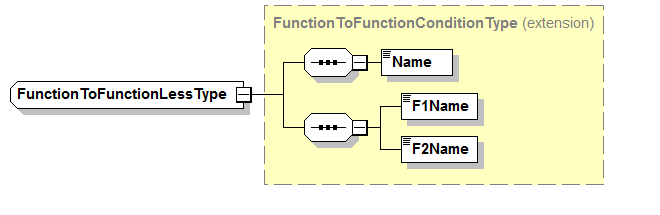
\includegraphics[width=8cm]{images/soap/FunctionToFunctionLessType.png}
\caption{Function to function less model.}
\label{fig:FunctionToFunctionLessType}
\end{figure}
\begin{figure}[htb!]
\centering
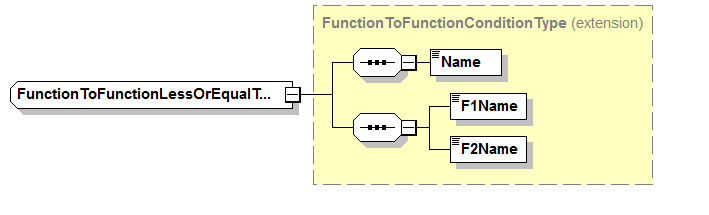
\includegraphics[width=8cm]{images/soap/FunctionToFunctionLessOrEqualType.png}
\caption{Function to function less or equal model.}
\label{fig:FunctionToFunctionLessOrEqualType}
\end{figure}
\begin{figure}[htb!]
\centering
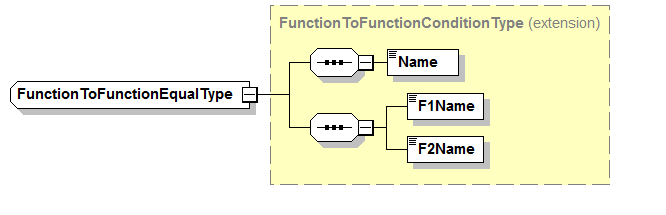
\includegraphics[width=8cm]{images/soap/FunctionToFunctionEqualType.png}
\caption{Function to function equal model.}
\label{fig:FunctionToFunctionEqualType}
\end{figure}
\begin{figure}[htb!]
\centering
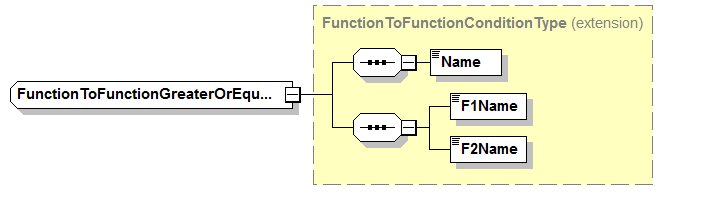
\includegraphics[width=8cm]{images/soap/FunctionToFunctionGreaterOrEqualType.png}
\caption{Function to function greater or equal model.}
\label{fig:FunctionToFunctionGreaterOrEqualType}
\end{figure}
\begin{figure}[htb!]
\centering
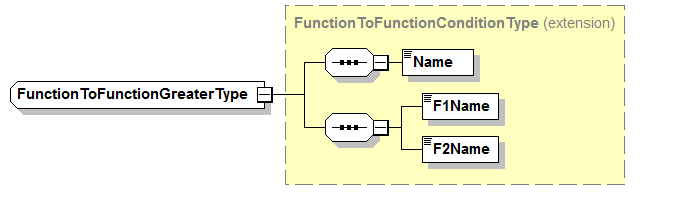
\includegraphics[width=8cm]{images/soap/FunctionToFunctionGreaterType.png}
\caption{Function to function greater model.}
\label{fig:FunctionToFunctionGreaterType}
\end{figure}


\begin{figure}[htb!]
\centering
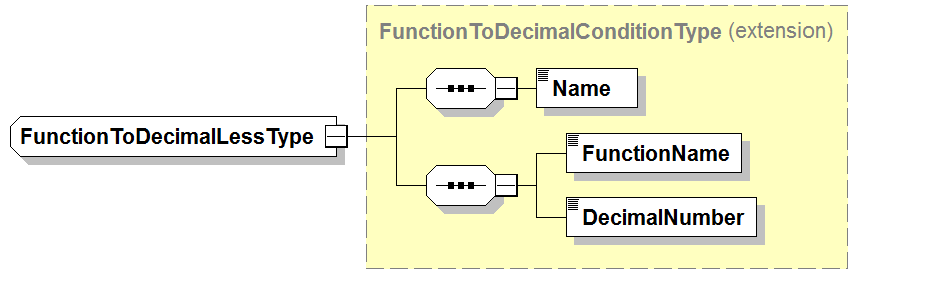
\includegraphics[width=8cm]{images/soap/FunctionToDecimalLessType.png}
\caption{Function to decimal less model.}
\label{fig:FunctionToDecimalLessType}
\end{figure}
\begin{figure}[htb!]
\centering
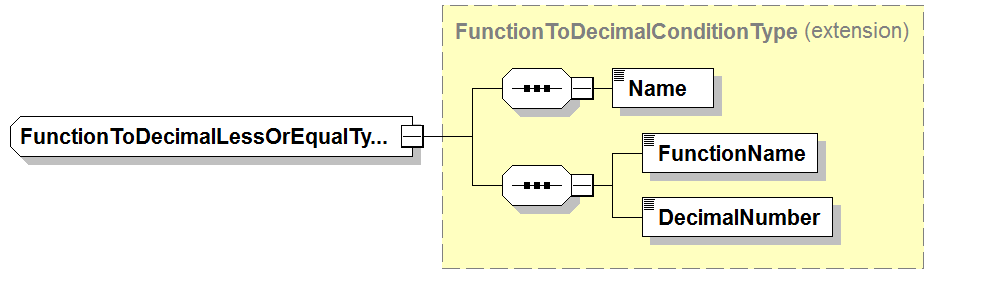
\includegraphics[width=8cm]{images/soap/FunctionToDecimalLessOrEqualType.png}
\caption{Function to decimal less or equal model.}
\label{fig:FunctionToDecimalLessOrEqualType}
\end{figure}
\begin{figure}[htb!]
\centering
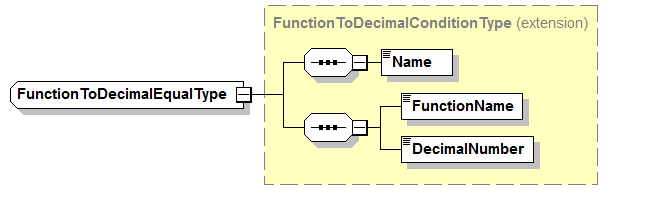
\includegraphics[width=8cm]{images/soap/FunctionToDecimalEqualType.png}
\caption{Function to decimal equal model.}
\label{fig:FunctionToDecimalEqualType}
\end{figure}
\begin{figure}[htb!]
\centering
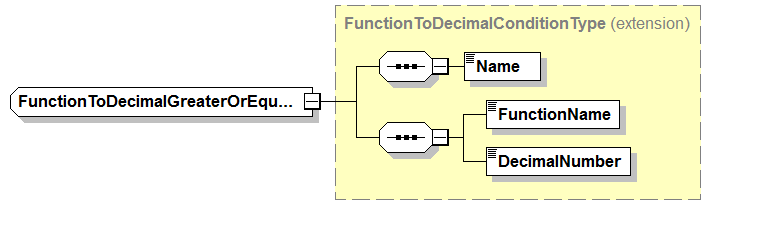
\includegraphics[width=8cm]{images/soap/FunctionToDecimalGreaterOrEqualType.png}
\caption{Function to decimal greater or equal model.}
\label{fig:FunctionToDecimalGreaterOrEqualType}
\end{figure}
\begin{figure}[htb!]
\centering
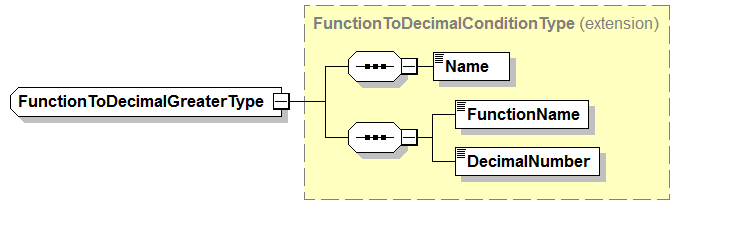
\includegraphics[width=8cm]{images/soap/FunctionToDecimalGreaterType.png}
\caption{Function to decimal greater model.}
\label{fig:FunctionToDecimalGreaterType}
\end{figure}


\begin{figure}[htb!]
\centering
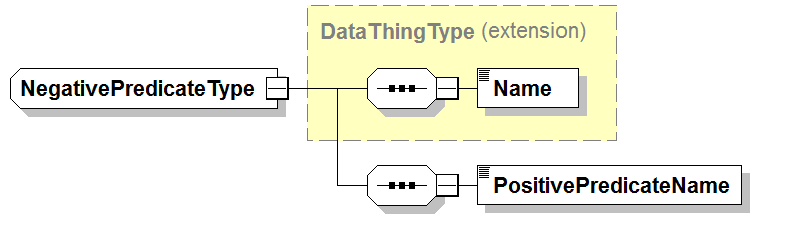
\includegraphics[width=8cm]{images/soap/NegativePredicateType.png}
\caption{Negative predicate model.}
\label{fig:NegativePredicateType}
\end{figure}

\begin{figure}[htb!]
\centering
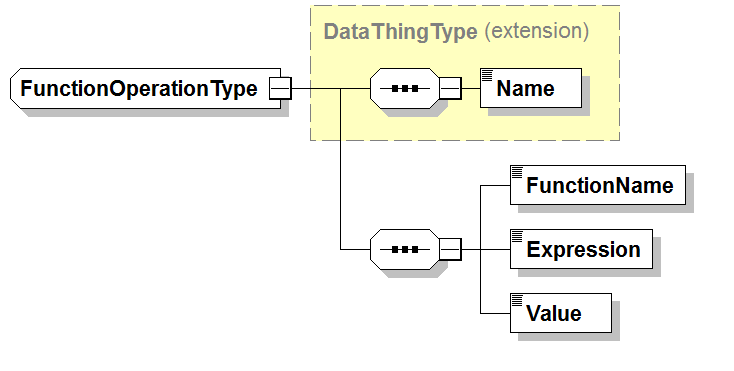
\includegraphics[width=8cm]{images/soap/FunctionOperationType.png}
\caption{Function operation model.}
\label{fig:FunctionOperationType}
\end{figure}


%
%\subsection{Hand Generation of SOAP XML Instance File}
%Once the SOAP XML schema model file in place, we developed a SOAP XML data file that conforms to the schema model. Under the XML standards, an XML data file conforming to an XML
%schema must be in a different format than the schema and must contain different sorts of statements. An XML statement naming the XML schema file to which an instance file corresponds is normally given near the beginning of the instance file. Many different instance files may correspond to the same schema. The form of an instance file is a tree in which instances of the elements of each type are textually inside the instance of the type. A sample of the hand generated XML file that conforms to the SOAP XML schema file is depicted in Figure~\ref{soapinstance}. We illustrated how the action take-kitTray is described in an XML form.

\section{Automatic Generation of PDDL Files}
\label{section:java-tool}
Once the schema models for PDDL in place, an XML instance file that conforms to the schema models was developed. Under the XML standards, an XML data file conforming to an XML schema must be in a different format than the schema and must contain different sorts of statements. An XML statement naming the XML schema file to which an instance file corresponds is normally given near the beginning of the instance file. Many different instance files may correspond to the same schema. The form of an instance file is a tree in which instances of the elements of each type are textually inside the instance of the type. Schema models and the XML instance file are used by a set of tools to automatically generate a set of OWL files. The tools required to perform this mechanism were developed by one of the authors at NIST. More information about this set of tools can be found in~\cite{Balakirsky.NISTIR.2013}.

To date, the PDDL domain and problem files are hand generated. An expert needs to write these two files and it takes a considerable amount of time to complete these files.
A Java-based tool presented was developed in this effort to automatically and dynamically build these PDDL files. The tool was developed in Java because of its inherent ability to interface with OWL API~\cite{OWLAPI}. The OWL API is a Java API and reference implementation for creating, manipulating
and serialising OWL Ontologies. Please note that the use of the language and the API is the authors' choice and the same result may be obtained differently.

\IncMargin{1em}
\begin{algorithm}
\SetKwData{Left}{left}
\SetKwData{This}{this}
\SetKwData{Up}{up}
\SetKwFunction{Union}{Union}
\SetKwFunction{FindCompress}{FindCompress}
\SetKwInOut{Input}{input}
\SetKwInOut{Output}{output}
\BlankLine
\emph{read OWLClass:PartsTray in OWL file}\;
\emph{build $partsTrayNodeSet=[partsTray_i]_{i=1}^{i=n}$}\;
\If(){$partsTrayNodeSet$ is not empty}{\For{each $partsTray_i$}{build $partNodeSet=[part_j:(kit_i,hasPartsVessel\_Part)]_{i=1,j=1}^{i=n,j=o}$\;
\If(){$partNodeSet$ is not empty}{
\For{each $part_j$}{write (hasPartsVessel-Part $partsTray_i$ $part_j$)$_{i=1, j=1}^{i=n, j=o}$}}}}

\caption{Dynamic building and writing of a predicate}\label{algo}
\end{algorithm}\DecMargin{1em}
The generation of the PDDL domain file is performed by reading the OWL classes from the SOAP OWL file that define PDDL structures. Since a PDDL domain file stays unchanged during a replanning process, the blueprint of the PDDL domain file is programmed. The tool only needs to access each part of this blueprint from the ontology and outputs this information in a PDDL domain file. The PDDL problem file, however, consists of a dynamically generated \textsf{init} state. This dynamic generation of the \textsf{init} state allows a successful replanning process where the current state of the world becomes the new \textsf{init} state of the problem file. The tool has the ability to read the SOAP OWL file and to write only predicates and function operations that satisfy the \textsf{init} state. In other words, a mapping for predicates and function operations is programmed and the tool writes predicates and function operations only if relevant information exists for those predicates and function operations.

For instance, the predicate \textsf{hasPartsVessel-Part part\_a\_tray part\_a\_1} (line 32 in Figure~\ref{fig:problem}) is true if the parts tray \textsf{part\_a\_tray} contains the part \textsf{part\_a\_1}. The process to build and write this predicate in the \textsf{init} section of the problem file is described in Figure~\ref{algo}. The different prerequisites for this predicate to be written in the \textsf{init} state of the problem file are described as follows. The tool reads the class PartsTray from an OWL init file, retrieves all the individuals in this class (line 1) and inserts them in $partsTrayNodeSet$ (line 2). If $partsTrayNodeSet$ is not empty (line 3), for each $partsTray$ (line 4) the tool uses the object property $hasPartsVessel\_Part$ to retrieve all the parts. The parts are then stored in $partNodeSet$ (line 5). If $partNodeSet$ is not empty (line 6), then the tool writes the predicate \textsf{partsVessel-has-part} with the correct name for the individuals (\textsf{part\_a\_tray} and \textsf{part\_a\_1} in our example). Note that if the condition at line 3 is not satisfied, i.e., if there is no parts trays in the ontology, this predicate is not written in the initial state of the problem file. Similarly, if $partNodeSet$ is empty, i.e., there is no parts in the parts tray, the predicate is also not written in the problem file.


%The process to build this predicate is as follows:
%	 * <ul>
%	 * <li>read <i>OWLClass:PartsTray</i> in OWL init file
%	 * <ul>
%	 * <li>build\f$partsTrayNodeSet=[partsTray_i]_{i=1}^{i=n}\f$
%	 * <ul>
%	 * <li>\f$\rightarrow\f$for each \f$partsTray_i\f$
%	 * <ul>
%	 * <li>build\f$partNodeSet=[part_j:(kit_i,hasPartsVessel\_Part)]_{i=1,j=1}^{i=n,j=o}\f$
%	 * <li>\f$\rightarrow\f$for each \f$part_j\f$
%	 * <ul>
%	 * <li>\f$\rightarrow\f$build (partsVessel-has-part\f$(partsTray_i\f$ \f$part_j\f$)\f$_{i=1, j=1}^{i=n, j=o}\f$
%	 * </ul>
%	 * </ul>
%	 * </ul>
%	 * </ul>
%	 * </ul>


\section{Conclusion and Future Work}
\label{section:conclusion}

This paper presented the latest tasks in the area of kit building, part of the "Agility Performance of Robotic Systems" project at the National Institute of Standards and Technology (NIST). The authors presented different models for PDDL structures. These models are used to generate a set of OWL files. The generated OWL files are employed to automatically and dynamically generate PDDL domain and problem files. This function allows a system to cope with failures with the production of new problem files based on the current state of the world. The automatic and dynamic generation of PDDL files is an attempt at bringing agility and flexibility in the current kitting system. As mentioned in Section~\ref{section:architecture}, a MySQL database is used to store information on the current state of the world. The next step in this effort is to generate PDDL files directly from the MySQL database which contains the latest snapshot of the world.
\section{Disclaimer}
No approval or endorsement of any commercial product by the authors is intended or implied. Certain commercial software systems are identified in this paper to facilitate understanding. Such identification does not imply that these software systems are necessarily the best available for the purpose.
%% The Appendices part is started with the command \appendix;
%% appendix sections are then done as normal sections
% \appendix
%
% \section{Test}
% \label{XMLInstance}
%
%\begin{mylisting}
%\begin{Verbatim}[commandchars=\\\{\},fontsize=\footnotesize,  numbersep=1pt]
%<TakeKitTray>
%    <Name>take-kitTray</Name>
%    <Description>;Take a KitTray from a LargeBoxWithEmptyKitTrays</Description>
%    <ActionParameterSet>
%        <Name>robot-TakeKitTray</Name>
%        <ActionParameter>Robot</ActionParameter>
%        <ActionParameterPosition>1</ActionParameterPosition>
%    </ActionParameterSet>
%    <ActionParameterSet>
%        <Name>kitTray-TakeKitTray</Name>
%        <ActionParameter>KitTray</ActionParameter>
%        <ActionParameterPosition>2</ActionParameterPosition>
%    </ActionParameterSet>
%    <ActionParameterSet>
%        <Name>lbwekt-TakeKitTray</Name>
%        <ActionParameter>LargeBoxWithEmptyKitTrays</ActionParameter>
%        <ActionParameterPosition>3</ActionParameterPosition>
%    </ActionParameterSet>
%    <ActionParameterSet>
%        <Name>endEffector-TakeKitTray</Name>
%        <ActionParameter>EndEffector</ActionParameter>
%        <ActionParameterPosition>4</ActionParameterPosition>
%    </ActionParameterSet>
%    <ActionParameterSet>
%        <Name>sku-TakeKitTray</Name>
%        <ActionParameter>StockKeepingUnit</ActionParameter>
%        <ActionParameterPosition>5</ActionParameterPosition>
%    </ActionParameterSet>
%    <Precondition>
%        <Name>precondition-TakeKitTray</Name>
%        <F2DGreaterTakeKitTray>
%          <Name>f2d-TakeKitTray</Name>
%          <DecimalNumber>0.000000</DecimalNumber>
%          <F1Name>quantity-of-kittrays-in-lbwekt</F1Name>
%        </F2DGreaterTakeKitTray>
%        <EEffHasNoObjectName>endEffector-has-no-heldObject</EEffHasNoObjectName>
%        <EEffIsForKitTraySKUName>endEffector-is-for-kitTraySKU</EEffIsForKitTraySKUName>
%        <EEffHasRobotName>endEffector-has-physicalLocation-refObject-robot</EEffHasRobotName>
%        <KitTrayHasSKUObjectSKUName>kitTray-has-skuObject-sku</KitTrayHasSKUObjectSKUName>
%        <KitTrayHasRefObjectLBWEKTName>kitTray-has-physicalLocation-refObject-lbwekt</KitTrayHasRefObjectLBWEKTName>
%        <RobotHasEEffName>robot-has-endEffector</RobotHasEEffName>
%    </Precondition>
%    <Effect>
%        <Name>effect-TakeKitTray</Name>
%        <FODecreaseTakeKitTray>
%          <Name>decrease-TakeKitTray</Name>
%          <Expression>decrease</Expression>
%          <Value>1</Value>
%          <FunctionName>quantity-of-kittrays-in-lbwekt</FunctionName>
%        </FODecreaseTakeKitTray>
%        <EEffHasKitTrayName>endEffector-has-heldObject-kitTray</EEffHasKitTrayName>
%        <KitTrayHasRefObjectEEffName>kitTray-has-physicalLocation-refObject-endEffector</KitTrayHasRefObjectEEffName>
%        <NotEEffHasNoObjectName>not-endEffector-has-no-heldObject</NotEEffHasNoObjectName>
%        <NotKitTrayHasRefObjectLBWEKTName>not-kitTray-has-physicalLocation-refObject-lbwekt</NotKitTrayHasRefObjectLBWEKTName>
%    </Effect>
%</TakeKitTray>
%\end{Verbatim}
%\captionof{figure}{Sample of SOAPInstance.xml file}
%\label{soapinstance}
%\end{mylisting}
%% References
%%
%% Following citation commands can be used in the body text:
%% Usage of \cite is as follows:
%%   \cite{key}         ==>>  [#]
%%   \cite[chap. 2]{key} ==>> [#, chap. 2]
%%

%% References with BibTeX database:

\bibliographystyle{elsarticle-num}
\bibliography{RCIM-KOOTBALLY}

%% Authors are advised to use a BibTeX database file for their reference list.
%% The provided style file elsarticle-num.bst formats references in the required Procedia style

%% For references without a BibTeX database:

% \begin{thebibliography}{00}

%% \bibitem must have the following form:
%%   \bibitem{key}...
%%

% \bibitem{}

% \end{thebibliography}

\end{document}

%%
%% End of file `ecrc-template.tex'. 